\documentclass{article}
\usepackage{datetime}
\usepackage{listings}
\usepackage{float} % To use the [H] option for figure placement
\usepackage{graphicx} % To include graphics
\usepackage{adjustbox} % For more flexible image adjustments

\title{LogBook Tesi}
\author{Kamil Laurent}

\begin{document}
\maketitle

\section*{Settimana del 25 marzo 2024}
\subsection{argomenti trattati}
\begin{itemize}
    \item Test di una forma funzionale complessa (MAP22g52) su una forma semplice (PV19 o PV17):
    assicurarsi che la parte di Hard Process (tabelle) sia la stessa usata per generare e fittare i dati, deve cambiare solo la parametrizzazione. 
    \item Se fittiamo i dati generati con la PV19, stiamo al N3LL, ci aspettiamo una parametrizzazione consistente per la PDF (Drell-Yan) e dei parametri casuali per la FF (SIDIS).
    \item se fittiamo dati generati con PV17, ci aspettiamo che questi pseudo-dati siano molto diversi dai dati reali, ma questo ci permette comunque di vedere se la procedura trova il minimo nello spazio dei parametri. In questo caso dobbiamo usare la parametrizzazione g52 con le tabelle al NLL.
    \item Closure Test L0: è utile vedere in che modo si comporta la replica 0 (non fluttuata), non ci interessano le altre repliche. Ci interessa comunque vedere come si comporta il minimizzatore se parto da un punto diverso nello spazio dei parametri
    
\end{itemize}

\subsection{da fare}
\begin{itemize}
    \item capire se ComputeMeanReplica ha senso
    \item fittare 20 volte la `replica 0` lasciando $Paramfluct = true$ nella card. Fare questo usando come minimizer sia ceres che minuit--> sembra che anche con Paramfluct = true il minimizer parta sempre dallo stesso punto nello spazio delle fasi. Provare a cambiare il seed.
    
    \item implementare un pezzo di codice che confronti i parametri trovati con i fit e quelli usati per generare i dati, qualcosa del tipo:
    \[ \sum_{i=1}^{21} \frac{|p_{i}^{fit} - p_{i}^{true}|}{p_i^{true}} \]
    dove $p_i$ è il parametro i-esimo della forma funzionale della TMD
    \item fare un CT L0 su dati generati da PV19. Usare 20 repliche come sopra e vedere il $\chi^2$ per la bontà del test. Qui non possiamo confrontare i parametri uno per uno, per cui vediamo se le forme delle TMD generate in Report coincidono.
    \item generare gli pseudo-dati L1 usando lo stesso file .py usato per i dati L0 che tenga in considerazione le incertezze sui dati sperimentali. I punti vengono generati con la formula:
    \[ d_i^{L1} = (1+\sum_{q=1}^{N_{norm}} r_q^{norm}\sigma_{q,i}^{norm})(t_i^0 + \sum_{p=1}^{N_{sys}} r_p^{sys}\sigma_{p,i}^{sys} + r_i^{unc} \sigma_i^{unc} )\]
    dove $t_i^0$ è il valore centrale teorico (senza incertezza) $r \in [-1,1]$ sono dei valori generati randomicamente da una distribuzione gaussiana (associati alle varie incertezze, sono dipendenti dal datapoint solo per le incertezze non correlate), $\sigma$ sono le incertezze, che possono essere correlate (di normalizzazione, norm, o sistematiche, sys) e non correlate, unc.
    Sui datasets che usiamo per i fit queste 3 forme di incertezza sono così mappate: norm = mult, unc = unc, sys = add.
\end{itemize}
\subsection{risultati}
\begin{itemize}
    \item MAP22 su MAP22 ceres: su 20 repliche, 16 hanno un $\chi^2 \propto O(e^{-14})$, 2 hanno $\chi^2 \propto O(e^{-6})$ e 2 hanno $\chi^2 \propto O(10^{-3})$.
    Sospetto che il minimizzatore si fermi anche se non ha trovato il minimo, nel caso in cui $\chi^2 \propto O(10^{-3})$ perché è soddisfatta la seguente condizione che si può vedere nel output del fit: 
    \begin{lstlisting}[language=bash]
    CONVERGENCE (Function tolerance reached.
    |cost_change|/cost: 2.554821e-06 <= 1.000000e-05)
    \end{lstlisting}

   \item MAP22 su MAP22 minuit: qui il range di valori del $\chi^2$ è più stretto ma i valori sono più distribuiti. In generale il $\chi^2$ è più alto rispetto al caso in cui si utilizza ceres

   \item MAP22 su PV19 Ceres: il $\chi^2$ varia ma è sempre di $O(10^{-1})$ in tutte le repliche, qui bisogna vedere i grafici delle TMD per farsi un'idea della bontà dei fit e della parametrizzazione.

   \item MAP22 su PV19 minuit: nessuna delle 20 repliche è arrivata a convergenza.

   \item creato il dataset L1 a partire da MAP22, fatto un primo fit (replica 0) a partire da questi dati con la parametrizzazione MAP22g52. In questo caso il $\chi^2$ è peggiore del caso L0 (ci aspettiamo che sia cosi)

   \item comparando la distribuzione della $f_{NP}(x, b_{T}, \zeta)$ con la parametrizzazione PV19 e con la parametrizzazione MAP22, ci aspettiamo che abbiano la stessa forma? 
   Dalla parametrizzazione PV19x otteniamo 9 parametri dai quali dipende la nostra distribuzione:

    \[ f_{\rm NP}(x, \zeta, b_T) = \left(\frac{1 - \lambda}{1 + g_1(x) \frac{b_T^2}{4}} + \lambda \exp\left(-\frac{g_{1B}(x) b_T^2}{4}\right)\right) \exp\left[-g_2 \log\left(\frac{\zeta}{Q_0^2}\right) \frac{b_T^2}{4} - g_{2B} \log\left(\frac{\zeta}{Q_0^2}\right) \frac{b_T^4}{4}\right] \]

    in cui: 
    \[
    g_1(x) = \frac{N_1}{x\sigma} \exp \left[ - \frac{\ln^2\left(\frac{x}{\alpha}\right)}{2 \sigma^2} \right]
    \]
    
    \[
    g_{1B}(x) = \frac{N_{1B}}{x\sigma_B} \exp\left[ - \frac{\ln^2\left(\frac{x}{\alpha_B}\right)}{2 \sigma_B^2} \right]
    \]

    La parte non perturbativa della PDF entra nella PDF "totale" in questo modo:

    \[
    \hat{f}_1(x, b_T; \mu, \zeta) = f_{NP}(x, b_T, \zeta) \hat{f}_1(x, b_*(b_T); \mu, \zeta)
    \]

    quest'ultima entra nella sezione d'urto (osservabile fisica) in questo modo:
    \[
    \frac{d \sigma}{dQ dy dq_T } = \frac{8\pi \alpha^2 q_T P}{9 Q^3} H(Q, \mu) \sum_q C_q(Q) \int_{0}^{\infty}db_T b_T J_0(b_Tq_T)x_1\hat{f}_1^q(x_1, b_T; \mu, \zeta) x_2\hat{f}_1^{\bar{q}}(x_2, b_T; \mu, \zeta)
    \]
    
    \item la parametrizzazione di MAP22 invece ha una forma funzionale diversa, data da 11 parametri (qui iserisco solo la parametrizzazione della $f_{NP}$ perché fittando dati ottenuti da Drell-Yan non stiamo fittando le fragmentation functions):
    
    \[
    f_{\rm NP}(x,\zeta, b_T)= \exp(S_{\rm NP}(\zeta, b_T))
    \]
    \[
    \frac{g_1(x) \exp( - g_1(x) \frac{b_T^2}{4}) + \lambda^2 g_{1B}^2(x) ( 1 - g_{1B}(x) \frac{b_T^2}{4}) \exp( - g_{1B}(x) \frac{b_T^2}{4}) + \lambda_2^2 g_{1C}(x) exp( - g_{1C}(x) \frac{b_T^2}{4}) }{  g_1(x) +  \lambda^2 g_{1B}^2(x) + \lambda_2^2 g_{1C}(x)}
    \]

    dove:
    \[
    S_{\rm NP} = \exp\left[ - g_2^2 \frac{b_T^2}{4} \log \big (\frac{\zeta}{Q_0^2}\big ) \right]
    \]

    \[
    g_{1,1B,1C}(x) = N_{1,1B,1C} \frac{x^{\sigma_{1,2,3}}(1-x)^{\alpha^2_{1,2,3}}}{\hat{x}^{\sigma_{1,2,3}}(1-\hat{x})^{\alpha^2_{1,2,3}}}
    \]

    \[ f_{\rm NP}(x, \zeta, b_T) = \frac{N_1}{x\sigma_1} \left(\frac{x^{2\sigma_1} (1 - x){2\alpha_1}}{0.1{2\sigma_1} (1 - 0.1)^{2\alpha_1}}\right) \]

   

    Sia in MAP22g52 che in PV19 abbiamo che $Q_0 = 1 GeV$, in MAP22 abbiamo $\hat{x} = 0.1 $

    Questa entra nella PDF "totale" in questo modo:
    
\end{itemize}
  
\subsection{domande}

\begin{itemize}
    \item cosa fa esattamente l'opzione $Paramfluct$ nella card di configurazione?
    \item piccole variazioni nella formula per la generazione degli pseudodati L1 (ad esempio ci sono più incertezze non correlate)
    \item al L1 vogliamo testare cose diverse. Con il test L0 ci siamo accorti che ceres funziona meglio. Continuiamo con ceres abbandonando minuit? Questa volta se faccio un fit su 50 repliche, queste vanno fluttuate o cambiamo solo il punto di partenza nello spazio dei paramtri? Per ora sto facendo 50 repliche tutte fluttuando la replica 0.
    \item pensavo che in qesto caso sarebbe utile testare i sisultati con e senza la $t_0$ prescription, è corretto?

    \item serve ancora fare un fit sugli pseudodati generati con PV19x o abbiamo già testato che la nostra parametrizzazione funziona su dati più semplici? --> serve ancora.
\end{itemize}

\section{Settimana del 8 aprile 2024}

\subsection{argomenti trattati}
\begin{itemize}
    \item \textbf{Parametrizzazioni PV19 e MAP22: } quando facciamo un fit usando la parametrizzazione MAP22 su dati generati da PV19, dovremmo ottenere la stessa forma funzionale della parte non perturbativa della TMD. Questo perché nulla cambia nella relazione tra la $f_{NP}$ e la sezione d'urto nei due articoli PV19 e MAP22. L'unica cosa che cambia è la parametrizzazione della $f_{NP}$.
    \item \textbf{generazione degli pseudo-dati L1: } c'era una imprecisione nel modo in cui venivano pesati gli errori dei datapoint per la generazione degli pseudo-dati. In particolare nei fattori $r_q$, $r_p$, $r_i$, i quali devono essere generati randomicamente da una distribuzione normale $N(0, 1)$. Questi non devono per forza essere 'pinzati' nell'intervallo $[-1, 1]$. Generare di nuovo gli pseudo-dati con la distribuzione corretta.
    \item \textbf{fit degli pseudo-dati L1: } Per il fit L1, anche in questo caso le repliche non devono fluttuare i dati, ma devono partire da punti diversi nello spazio dei parametri. Ci aspettiamo che la distribuzione del $\chi ^2$ sia intorno a $1$. Qui vorremmo testare le seguenti cose:
    \begin{itemize}
        \item parametrizzazione MAP22 su pseudodati generati da PV19
        \item MAP22 su dati generati da MAP22 (procedura standard)
        \item MAP22 su MAP22 con la $t_0$ prescription
        \item altro?
    \end{itemize}
    
    \end{itemize}
    \subsection{da fare}
    \begin{itemize}
        \item Fare più repliche del fit con dati non fluttuati (50-100 invece di 20)
        \item provare con queste 100 repliche a rifare il fit e fare un plot di tutti i risultati che includa:
        \begin{itemize}
            \item la parametrizzazione con cui sono stati generati i dati (distribuzione \textbf{vera})
            \item le 100 distribuzioni ottenute con il fit.
        \end{itemize}
        \item capire perché il $\chi^2$ al L1 viene intorno a 2.45, a questo proposito farò 100 repliche con i dati che ho generato con un apposito codice e 100 repliche in cui uso la replica 9 (che in teoria dovrebbe essere fluttuata in qualche modo su cui non ho il controllo) cambiando in ogni replica il punto di partenza nello spazio dei parametri.
    \end{itemize}

    \subsection{risultati}
    \begin{itemize}
        \item I nuovi dati generati a una distribuzione normale $N(0,1)$ danno un $\chi^2 \tilde= 2.5 $, che è molto alto rispetto a quello che ci aspettiamo. Potrebbe esserci un errore in come il codice per la generazione degli pseudo-dati è stato implementato oppure nella distribuzione utilizzata
        \item ho fatto un test usando 100 volte la replica 9, qui mi è venuta una $error_function = E \tilde= 1$, che è quello che ci aspettiamo. il $\chi^2$ è molto piccolo e diverso dalla $E$ perché probabilmente la $E$ viene calcolata sui dati fluttuati, mentre il $\chi^2$ è calcolato sui dati non fluttuati.
        
    \end{itemize}
\section{Settimana del 15 aprile 2024}

    \subsection{argomenti trattati}
    \begin{itemize}
        \item Discusso degli argomenti della settimana scorsa
        \item g52 su PV19: troviamo 2 classi di funzioni, una vicina alla distribuzione vera, una abbastanza lontana. Capire se quella più vicina da un buon risultato.
        \item test L1: il test sembra funzionare se uso dati fluttuati da NangaParbat, non funziona se uso un codice a parte per aggiungere delle fluttuazioni sui dati usati in L0, capire perché
    \end{itemize}
    \subsection{da fare}
    \begin{itemize}
        \item g52 su PV19: implementare nel codice che genera il fit una parte che calcoli la distanza di una distribuzione dalla distribuzione vera
        \item closure test L1: forse quello che sbaglio è definire dei nuovi pesi per gli errori moltiplicativi e sistematici ad ogni sotto-dataset dell'esperimento e non a tutto l'esperimento. Ad esempio prendiamo l'esperimento E605: i dataset di questo esperimento sono divisi in 5 file, che corrispondono a dati presi per diversi valori di Q. Al momento il codice definisce dei pesi $r_{norm}$ e $r_{sys}$ ad ogni nuovo file, provo a definirli una volta sola per tutto l'esperimento E605. NO
        \item qui: https://arxiv.org/pdf/0808.1231.pdf (formule 13 e 14) viene spiegato come generare le repliche Monte Carlo per un certo dataset. Questo è il modo in cui vengono generate le repliche in Nanga Parbat. In questo paper viene specificato che anche la matrice di covarianza viene cambiata (le incertezze vengono riscalate), questo è analogo a fare il fit con la $t_0$ prescription e le incertezze non riscalate? 
    \end{itemize}

    \subsection{Risultati}
    \begin{itemize}
        \item Fluttuare allo stesso modo tutti i dati per un certo esperimento non ha prodotto risultati buoni, il $\chi^2$ rimane molto alto
        \item fare un fit L1 con la $t_0$ prescription attiva 
        \item g52 su PV19 al L0: ho implementato una condizone sulla distanza media in quadratura di una certa distribuzione ottenuta dal fit dalla distribuzione vera. Chiamo Mean Squared Distance la distanza:
        \[ MSD = \frac{1}{N_{points}} \sum_{i = 1}^{N_{points}} (f_{NP, i}^{pred} - f_{NP, i}^{real})^2\]

        Ottengo: 
        \begin{itemize}
            \item $MSD < 0.0001$ per 0 repliche ( $0 \% $)
            \item $MSD < 0.0005$ per 47 repliche  ($47 \% $)
            \item $MSD < 0.01$ per 52 repliche  ($52 \% $)
        \end{itemize}
    \end{itemize}

\section{Settimana del 22 aprile 2024}

\subsection{Argomenti trattati}
\begin{itemize}
    \item MAP22g52 su PV19: test al L0 quasi concluso, troviamo due classi di funzioni, una delle quali approssima bene la distribuzione vera, una no. Circa nel $50 \%$ dei casi troviamo una distribuzione che approssima quella vera. 
    Prossimi passi:
    \begin{itemize}
        \item verificare cosa succede al L1
        \item esplorare il comportamento di una parametrizzazione più libera, come una rete neurale. In questo caso mi aspetto che la distribuzione vera sia riprodotta correttamente in più repliche rispetto al caso della parametrizzazione MAP22g52.
        \item si può pensare di utilizzare la parametrizzazione MAP24
    \end{itemize}

    \item La formula per la generazione degli pseudo-dati L1 scritta in precedenza è sbagliata. Dobbiamo tenere in considerazione due cose: 
    \begin{itemize}
        \item ci sono due tipo di incertezze nei datasets (assolute e relative). Per prima cosa dobbiamo convertire tutte le incertezze in assolute 
        \item le incertezze moltiplicative vanno trattate come tali (vedi formula aggiornata sotto)
    \end{itemize}
    La formula corretta da usare è la seguente:
    \[
    d_i^{L1} = \prod_{q=1}^{N_{norm}}(1+ r_q^{norm}\sigma_{q,i}^{norm})(t_i^0 + \sum_{p=1}^{N_{sys}} r_p^{sys}\sigma_{p,i}^{sys} + r_i^{unc} \sigma_i^{unc} )
    \]
    \item Provare a fare un fit con la parametrizzazione PV19 su dati MAP22 come esercizio. Mi aspetto che il closure test non chiuda o che chiuda peggio di quanto non faccia con il setup opposto.
    \item incertezze sperimentali: nei file di dati ci sono 3 tipi di incertezze, \textit{unc}, \textit{mult} e \textit{add}, le ultime due sono relative e sono da convertire in incertezze assolute.

    
\end{itemize}
\subsection{risultati}

\subsection{domande}

\section{Settimana del 29 aprile 2024}

\subsection{Argomenti trattati}
\begin{itemize}
    \item \textbf{parametrizzazione PV19 su MAP22: } la parametrizzazione sembra funzionare molto bene, anche se abbiamo una discrepanza elevata in condizioni particolari. Ad esempio quando scegliamo di fare un plot della TMD a $Q = 1 GeV$ e $x = 0.1$, la parte non perturbativa ha un comportamento non fisico per grandi $b_T$ (dovrebbe andare a 0 ma non lo fa). Per contro il fit riproduce molto bene i nostri dati sperimentali, per cui la parametrizzazione funziona molto bene nelle regioni cinematiche in cui abbiamo preso i nostri dati sperimentali. 

    \item \textbf{fit in diverse condizioni: } Visto che il fit funziona molto bene ad energie dell'ordine di grandezza di $10 GeV$, provare a plottare le TMD della distribuzione vera e di quelle ottenute sia nel caso MAP22oPV19 che nel caso PV19oMAP22. Vedere nella regione cinematica considerata quale fit chiude meglio (contando che rispetto a MAP22oMAP22 nessuno dei due chiude al L0) 
    \item  \textbf{tabelle e testo: } fare delle tabelle con i risultati ottenuti fino ad ora e accompagnarle da alcuni paragrafi per spiegare il tutto. Cosa inserire:
    
    \begin{itemize}
        \item $\chi^2$ di: $L0MAP22oMAP22$, $L0PV19oMAP22$ e $L0MAP22oPV19$.
        \item $MSD$ (= Mean Squared Distance) dei plot delle TMD a $x = 0.1$, $Q = 10 GeV$ di $L0PV19oMAP22$  e $L0MAP22oPV19$
    \end{itemize}

    \item \textbf{Dati per l'esecuzione dei fit: } La differenza principale tra le parametrizzazioni MAP22g52 e PV19 sta nel fatto che MAP22 è un fit globale fatto su esperimenti di DY e SIDIS. Per cui la forma funzionale della TMD può essere usata anche per riprodurre dati sperimentali di SIDIS, cosa che non può essere fatta con la TMD di PV19. 
    Dovremmo provare a riprodurre anche dati L0 di tipo SIDIS partendo dalla TMD con la parametrizzazione PV19 e una FF nota che mettiamo noi dall'esterno, e vedere in che modo si comporta MAP22g52 su questo dataset.
    
    \item \textbf{L1: } ancora dei problemi sulla generazione dei dataset L1, capire cosa non va.
\end{itemize}
\subsection{risultati}
\begin{itemize}
    \item \textbf{ dati L1: } La formula per l'implementazione di dati L1 viene presa dal modo in cui Nanga Parbat genera le repliche e usata su un dataset L0 (perfetto-non fluttuato). L'implemetazione è la seguente:
    \[
    t_{L1}^i = t_0^1 \prod_{j=1}^{N_{norm}} \sqrt{(1 + r^{mult}_{j} \sigma_{i, j}^{mult})} (1 + \sum_{j=1}^{N_{norm}} r^{add}_{j} \sigma_{i, j}^{add} + r^{unc}_{j} \sigma_{i}^{unc}) 
    \]
    dove $\sigma_{i}^{unc} = \sqrt{\sum_{j=1}^{N_{unc}} \sigma_{i,j}^2}$. Gli errori in questa formula sono relativi, per cui convertiamo l'incertezza non correlata. 

    Lo faccio in due modi diversi: fluttuando le predizioni ottenute al livello 0, oppure partendo dai dati sperimentali, generando le predizioni direttamente da li. L'unica differenza sarà nel  modo in cui le incertezze non correlate vengono convertite in incertezze relative (nel primo caso $\sigma_{i}^{unc}/t_0$, nel secondo caso $\sigma_{i}^{unc}/t_{exp}$)

    \item \textbf{Nuovo Dataset: } 
\end{itemize}


\subsection{domande}

\section{Settimana del 27 maggio 2024}
\subsection{argomenti discussi}
\begin{itemize}
    \item confronto tra pseudodati generati con Nanga Parbat e generati con un codice a parte:
    \begin{figure}[H]
        \centering
        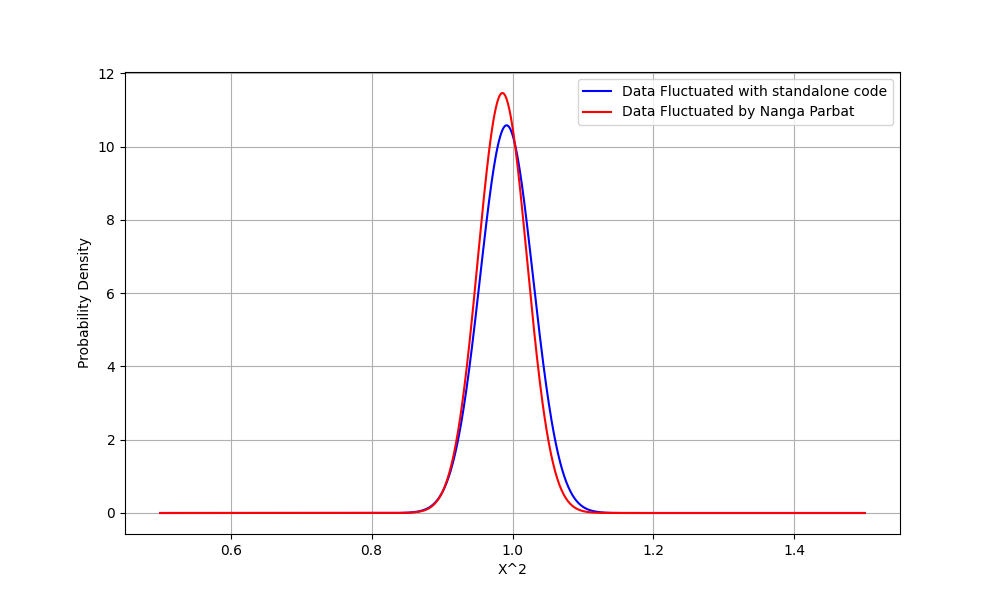
\includegraphics[width=0.9\textwidth]{Images/X2_distribution.png}
        \caption{distribuzione $\chi^2$ }
        \label{fig:enter-label}
    \end{figure}

    Credo che questa differenza (molto piccola) sia dovuta ai dati di Drell-Yan, alcuni dei quali hanno errori e valori centrali molto piccoli. In particolare credo che la causa sia il modo in cui python e C++ trattano i numeri molto piccoli. Infatti dobbiamo togliere dei datasets (Phoenix, D0 Run II e Run II $\mu$, Atlas a 8, 13 $TeV$, LHCb 7 e 13 $TeV$) quando usiamo python per effettuare la Cholesky decomposition, altrimenti si lamenta che la matrice di covarianza per questi datasets non è definita positiva.

    \item L1 tests: 
    ecco una tabella dei test al livello 1:
    \begin{table}[h]
    \caption{L1 results}
    \label{tab:L0_results}
    \centering
    \begin{adjustbox}{width=\textwidth}
        \begin{tabular}{|c|c|c|c|}
        \hline
        \textbf{name} & \textbf{fit parametrizetion:} & \textbf{pseudo-data  generated with:} & \textbf{mean $\chi^2$}\\
        \hline
        g52oMAP22 & MAP22g52 & MAP22g52 & da fare  \\
        PV19oPV19 & PV19x & PV19x & $0.9947 \pm 0.0002$  \\
        g52oPV19 & MAP22g52 &  PV19x & $1.3203 \pm 0.246$ \\
        PV19oMAP22 & PV19x & MAP22g52 &  $0.8424 \pm 0.0013$ \\
        \hline
    \end{tabular}
\end{adjustbox}
\end{table}
\end{itemize}
\section{Settimana del 3 giugno 2024}
\subsection{argomenti discussi}
\begin{itemize}
    \item Test della procedura di generazione dei dati al L1:
    Ho provato a generare 100 repliche dei dati Drell-Yan L1, ogni volta fluttuati in modo diverso. Cambiando solamente il modo in cui vengono fluttualti i dati e nient'altro otteniamo risultati molto diversi. Gli istogrammi sotto riportano il $\chi^2$ della replica 0 su 100 set di dati fluttuati in modo diverso (casuale). I test fatti fino ad ora sono:
    \begin{itemize}
        \item L1 con il metodo di fluttuazione "tradizionale" (python):
        \begin{figure}[H]
        \centering
        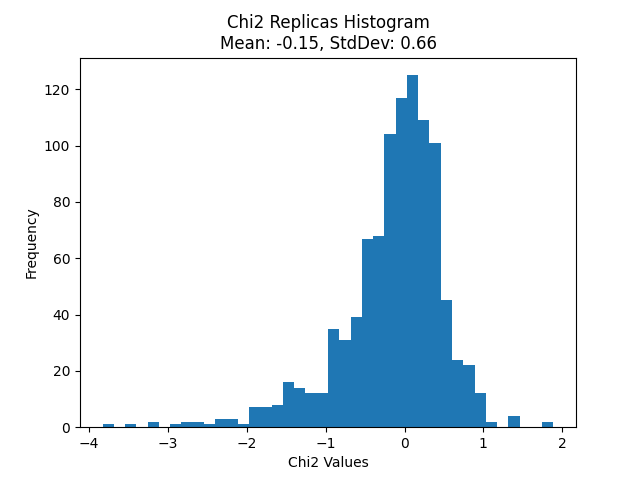
\includegraphics[width=0.5\textwidth]{Images/D0_X^2_distribution.png}
        \caption{$\chi^2 = 0.8333 \pm 0.0727$ }
        \label{fig:enter-label}
        \end{figure}

        \item L1, Cholesky decomposition, usando Numpy (i dataset che davano problemi sono stati fluttuati usando il metodo 'tradizionale')
        
        \begin{figure}[H]
        \centering
        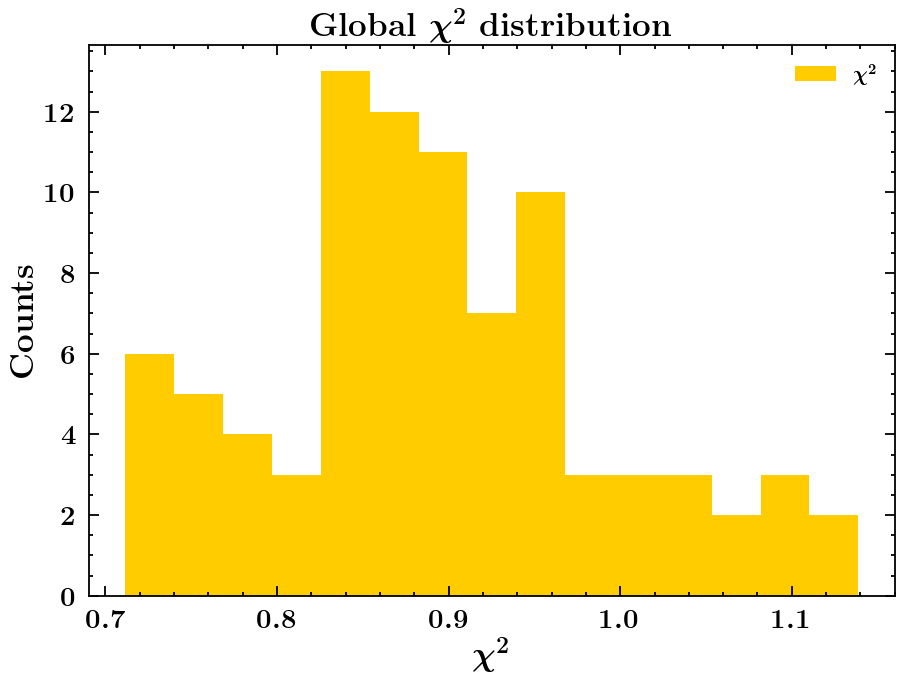
\includegraphics[width=0.5\textwidth]{Images/Globalchi2Numpy.png}
        \caption{$\chi^2 = 0.8935 \pm 0.0992$ }
        \label{fig:enter-label}
        \end{figure} 

        \item L1, Cholesky decomposition, usando Scipy (i dataset che davano problemi sono stati fluttuati usando il metodo 'tradizionale')
               
        \begin{figure}[H]
        \centering
        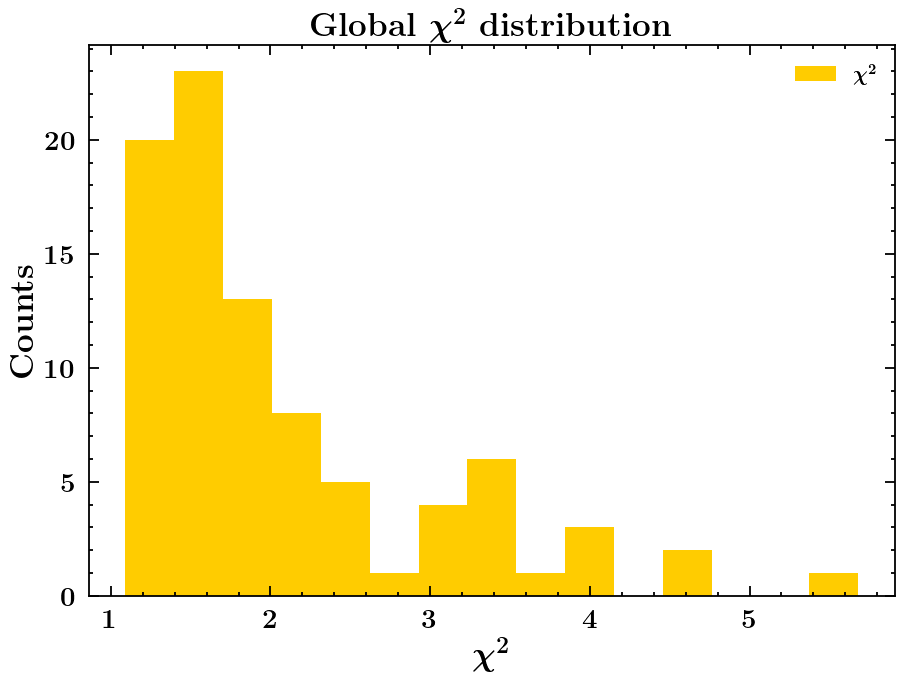
\includegraphics[width=0.5\textwidth]{Images/Globalchi2Scipy.png}
        \caption{$\chi^2 = 2.0617 \pm 0.9322$ }
        \label{fig:enter-label}
        \end{figure} 

        \item L1, Cholesky decomposition, usando Eigen (C++) (nessun dataset ha dato problemi)
               
        \begin{figure}[H]
        \centering
        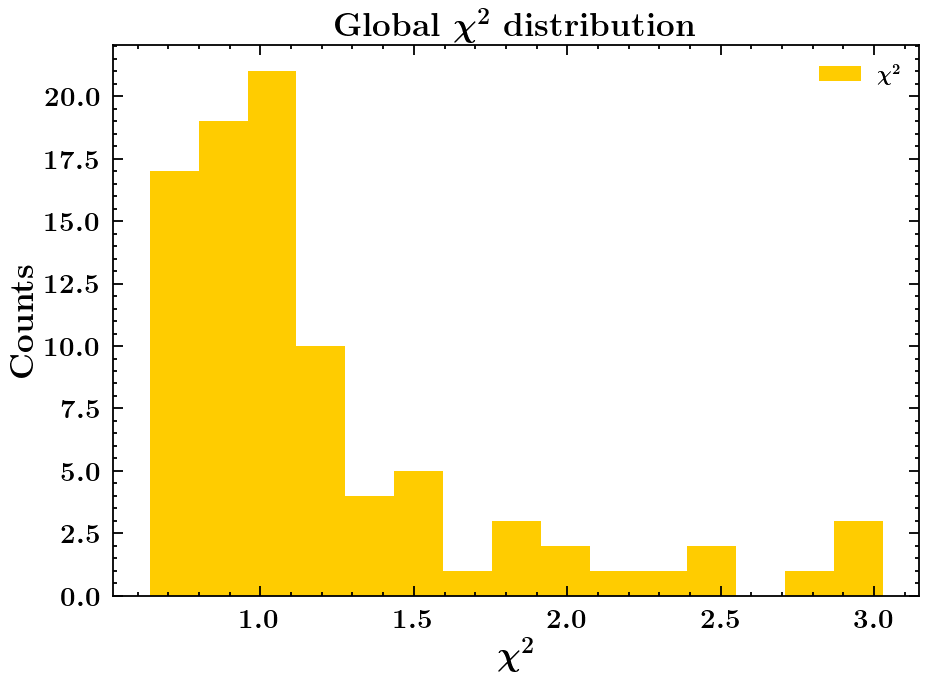
\includegraphics[width=0.5\textwidth]{Images/Globalchi2Eigen.png}
        \caption{$\chi^2 = 1.1871 \pm 0.5471$ }
        \label{fig:enter-label}
        \end{figure} 

        
    \end{itemize}

    \item L0 sulla parametrizzazione mista:
    ho generato delle predizioni da un fit sui dati usando le PDF di PV19 e le FF di MAP22. Dopodiché ho provato a ottenere nuovaente la distribuzione MIX24 sia con MAP22 che con PV19. Qui ci sono i risultati dei test su MIX24

    \begin{table}[h]
    \caption{L0 su MIX24}
    \label{tab:L0_results}
    \centering
    \begin{adjustbox}{width=\textwidth}
        \begin{tabular}{|c|c|c|c|}
        \hline
        \textbf{name} & \textbf{fit parametrization:} & \textbf{pseudo-data  generated with:} & \textbf{mean $\chi^2$}\\
        \hline
        $L0_g52oMIX24$ & MAP22g52 & MIX24 & $0.1546 \pm 0.0049$  \\
        $L0_PV19oMIX24$ & PV19x & MIX24 & $10^{-7}$  \\
        $L0_MIX24oMIX24$ & MIX24 & MIX24 & $0.0054 \pm 0.0045$ \\

        \hline
    \end{tabular}
\end{adjustbox}
\end{table}
\item Test L1 su due repliche di pseudo-dati diversi: ottengo due distribuzioni piccate su valori centrali diversi, a seconda del tipo di distribuzione che prendo
\end{itemize}
\subsection{Da fare}
\begin{itemize}
    \item \textbf{check della fluttuazione dei dati L1: } per assicurarsi che i dati L1 siano fluttuati correttamente, faccialo il seguente test:
    \begin{itemize}
        \item prendo i dati L0 e li fluttuo 100 volte (con il metodo che preferisco). Ottengo 100 repliche di dati fluttuati L1. Ad esempio consideriamo un singolo dataset (E605) al livello 0, l'i-esimo punto sarà  $t_i^0$. Ogni punto avrà adesso 100 repliche associate $t_{i,j}^1$ con $j=1, 2, ..., 100$
        \item per ogni dato sperimentale di queste 100 repliche calcolo il valore medio 'orizzontalmente' su queste 100 repliche: $<t_i^1> = \sum_{j=1}^{100}\frac{t_{i,j}^1}{100}$. Se il codice è giusto devo avere:
        \[ t_i^0 = <t_i^1>\]
        \item posso calcolare anche le incertezze correlate e non correlate (costruendo la matrice di covarianza dei dati?), ma non ho capito bene come fare        
    \end{itemize}

    \item \textbf{$L0-MIX24oMAP22$:} verificare che cosa succede se faccio un fit L0 con la parametrizzazione MIX24 (che ha le PDF di PV19 e le FF di MAP22g52) sui dati di MAP22. 
\end{itemize}

\subsection{Risultati}
\begin{itemize}
    \item \textbf{Test sulla generazione degli pseudodati: } Per prima cosa testiamo i vari metodi con una condizione sulle discrepanze dei valori medi:
    \[ \delta_i = \frac{| t_i^0 - <t_i^1>|}{t_i^0} \]
    \begin{table}[h]
    \caption{numero di punti non convergenti su 100 repliche genrate con differenti metodi}
    \label{tab:Distanza dal punto medio}
    \centering
    \begin{adjustbox}{width=\textwidth}
        \begin{tabular}{|c|c|c|c|}
        \hline
        \textbf{method} & \textbf{number of $\delta > 0.01$} & \textbf{$\delta > 0.02$} & \textbf{$\delta > 0.05$}\\
        \hline
        traditional  & 122 & 71 &  10 \\
        Cholesky, numpy & 139 & 81 & 14  \\
        Cholesky, scipy & 122 & 74 & 16 \\
        Cholesky, eigen & 106 & 69 & 9 \\
        \hline
    \end{tabular}
\end{adjustbox}
\end{table}
    Ho verificato che anche i punti con una discrepanza piuttosto alta, se aumento il numero di repliche drasticamente, torno alla media "vera" \\
    Per quanto riguarda la deviazione standard, ottengo una $\sigma_i$ dalla distribuzione dei dati fluttuati e la confronto con
    \[ \sigma_i = \sqrt{\sigma_{unc}^2 + (t_i^0 \sigma_{add})^2 + (t_i^0 \sigma_{mult})^2 }\]
    Facendo lo stesso test fatto per la media ottengo molti punti (decine o in alcuni casi centinaia) con una $\sigma$ piuttosto diversa da quella di partenza ($\delta_{\sigma} > 0.1$)
    \item \textbf{test $\chi^2$ sulle fluttuazioni: } posso verificare che le fluttuazioni siano costruite in modo perfetto (Gaussiano con le corrette $\sigma$) calcolando il $\chi^2$ tra la distribuzione dei dati fluttuati (L1) e la distribuzioni dei dati veri.
    \[ <\chi^2> = \frac{1}{N_{dat}} \sum_{i=1}^{N_dat}\frac{(t_i^0 - t_i^1)^2}{\sigma_i^2} \]

    Da questo test si vede chiaramente come alcuni dataset danno dei problemi. In particolare i dataset problematici sono: D0, PHENIX, LHCb. Comunque vengano fluttuati, questi danno una distribuzione del $\chi^2$ strana (vedi , dando origine anche a valori negativi. Questi valori negativi e le distribuzioni strane sono dovute molto probabilmente alle matrici di covarianza che secondo python non sono definite positive.
    \begin{figure}[H]
    \centering
    \begin{minipage}{0.45\textwidth}
        \centering
        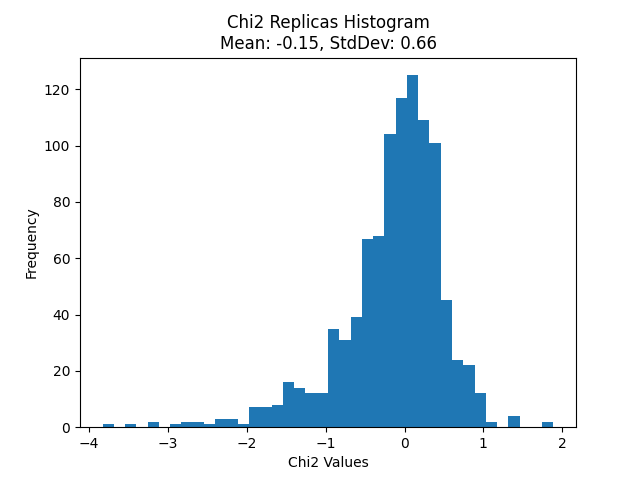
\includegraphics[width=\textwidth]{Images/D0_X^2_distribution.png}
        \caption{$\chi^2$ distribution of D0 replicas}
    \end{minipage}\hfill
    \begin{minipage}{0.45\textwidth}
        \centering
        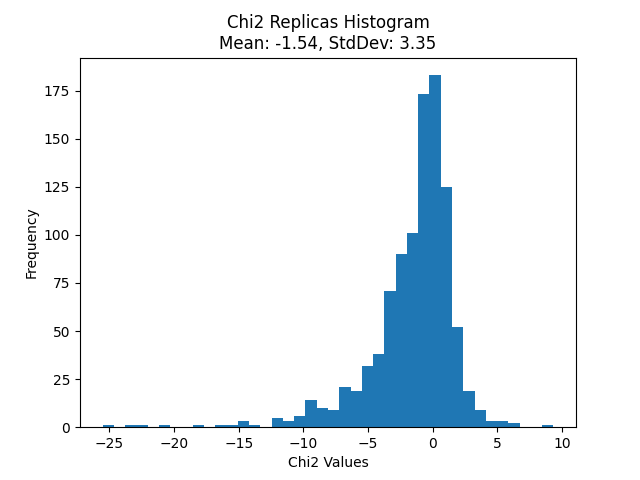
\includegraphics[width=\textwidth]{Images/LHCb_X^2_distribution.png}
        \caption{$\chi^2$ distribution of LHCb replicas}
    \end{minipage}
    \caption{some nonsense $\chi^2$ distribution}
    \end{figure}

    Ecco un confronto tra la distribuzione del $\chi^2$ medio su 1000 repliche con e senza i dataset problematici:
    \begin{figure}[H]
    \centering
    \begin{minipage}{0.45\textwidth}
        \centering
        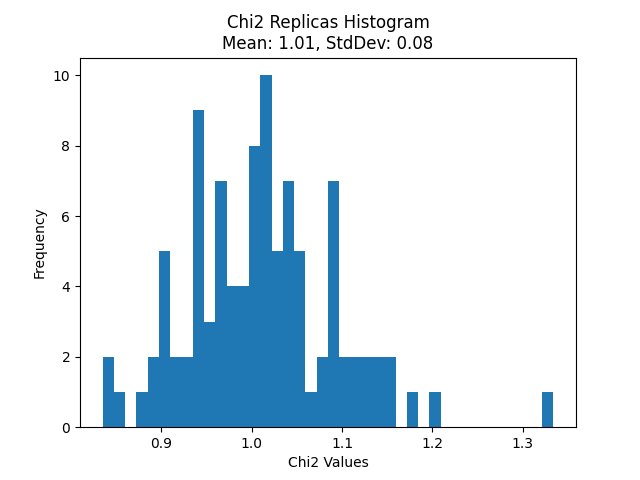
\includegraphics[width=\textwidth]{Images/Subset_X^2_distribution.png}
        \caption{$\chi^2$ distribution excluding DO, PHENIX, LHCb}
    \end{minipage}\hfill
    \begin{minipage}{0.45\textwidth}
        \centering
        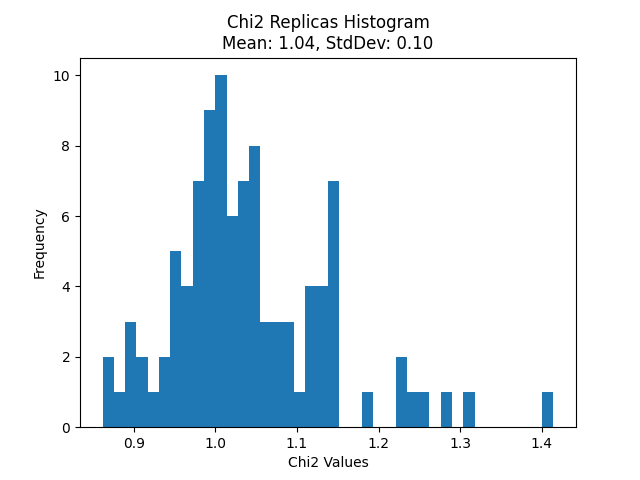
\includegraphics[width=\textwidth]{Images/X^2_distribution_2.png}
        \caption{$\chi^2$ of the complete dataset with prescriptions}
    \end{minipage}
    \caption{$\chi^2$ distribution tests}
    \end{figure}

    Propongo questa soluzione: genero insieme le fluttuazioni di tutti i dati che non danno problemi, fatto questo genero le fluttuazioni dei datasets problematici in maniera controllata, implementando delle condizioni sul $\chi^2$ medio
\end{itemize}

\section{Settimana del 17 giugno 2024}
\subsection{Discussioni della settimana precedente:}
\begin{itemize}
    \item \textbf{Generazione dati L1: } la questione è delicata perché non siamo ancora sicuri che tutti i punti siano fluttuati correttamente (senza errori numerici).
    
    \item Come gestiamo quei punti che essendo fluttuati assumono dei valori negativi? N.B. Nanga Parbat non ha un modo per gestire questi punti. Un buon modo per eliminare queso problema può essere questo: ogni volta che si presenta un numero negativo, rifacciamo tutta la fluttuazione del dataset, fino a che tutti i datapoint non diventano positivi
\end{itemize}
\subsection{risultati}
\begin{itemize}
    \item \textbf{Test L1 su 6 repliche: } prendiamo 6 repliche di dati fluttuati al L1 (usando Eigen, C++). Per ognuna di queste repliche faccio 50 fit senza fluttuare ulteriormente i dati, partendo da 50 punti diversi dello spazio dei parametri. A priori conosciamo il $\chi^2$ dei dati fluttuati rispetto ai dati "reali" ($<\chi^2>_{L0-L1}$), mentre il fit ci dice il $\chi^2$  della distribuzione ottenuta rispetto ai dati fluttuati ($<\chi^2>_{L1-fit}$). La tabella sotto riassume il valore di questi due stimatori statistici per le 6 repliche

    
    \begin{table}[h]
    \caption{L1 fluctuations with Eigen}
    \label{tab:L0_results}
    \centering
    \begin{adjustbox}{width=\textwidth}
        \begin{tabular}{|c|c|c|}
        \hline
        \textbf{replica} & \textbf{$<\chi^2>_{L0-L1}$} & \textbf{$<\chi^2>_{L1-fit}$} \\
        \hline
         0 & 0.921024 & 0.5743  \\
         1 & 1.03024 & 0.8257 \\
         2 & 0.965785 & 0.7304 \\
         3 & 0.980609 & 0.7449 \\
         4 & 0.744909  & 0.5027 \\
         5 & 1.20093 & 1.0048 \\
        \hline
    \end{tabular}
\end{adjustbox}
\end{table}
\item \textbf{stesso test fatto per g52oMAP22} In questo caso specifico abbiamo un risultato più incoraggiante 
\end{itemize}

\subsection{da fare:}
\begin{itemize}
    

\item \textbf{Repliche dei datasets al L1:} abbiamo adesso 6 repliche di dati fluttuati in modo diverso (riproducibile con un seed). Concludiamo il fit al L1 su chiascuna di queste 6 repliche.

\item \textbf{test L2 g52oMAP22}: scegliere una delle 6 repliche fluttuate al L1 e fare un test L2

\item \textbf{Incertezze su g52oMAP22} quando abbiamo tutti questi fit, faciamo un plot delle incertezze delle TMD ottenute:
\begin{itemize}
    \item incertzze di interpolazione
    \item incertezze funzionali
    \item incertezze sperimentali
\end{itemize}
\end{itemize}
\section{Settimana del 25 giugno 2024}
\subsection{Argomenti discussi}
\begin{itemize}
    \item \textbf{test L0: } abbiamo concluso i test al livello 0 e gli unici test che riusciamo a portare a chiusura sono g52oMAP22 e PV19oPV19. Questo significa che le nostre parametrizzazioni funzionano bene nel caso in cui la legge utilizzata sia molto simile alla legge vera, il che è poco probabile.
    \item \textbf{Caratterizzazione delle incertezze: } ci sono diversi modi per generare dei plot che tengano in considerazione le incertezze, il modo più semplice è quello di plottare punto per punto le bande d'errore usando media e deviazione standard del vettore che riempio con i valori delle $f_{NP}$, ma in questo modo ottengo una banda d'errore piccola e non riesco a distinguere con chiarezza le incertezze del L1 e del L2.\\ Un secondo modo è quello di plottare i rapporti:
    \[ \frac{f_{NP, true}}{f_{NP, pred}}\] avendo così una media e una deviazione standard del vettore contenente questi rapporti.
    \item \textbf{componenti delle incertezze: } possiamo fare il plot di media e deviazione standard nei 3 casi (L0, L1, L2) e confrontare i livelli di incertezze di interpolazione/estrapolazione, funzionali e sperimentali facendo i rapporti di queste incertezze. In questo modo possiamo accorgerci dei contributi di ogni tipo di incertezza all'incertezza totale. 
    \item \textbf{migliore visualizzazione delle incertezze: } Provare a ripetere lo stesso plot a scale di energie più basse ($Q = 1GeV$) e basso $x$ ($x < 0.1$). Ci aspettiamo che l'incertezza cresca e si possa vedere più chiaramente.
    \item  \textbf{Metà tesi: } la probabile data della metà tesi è il 22 luglio, commissario esterno: Miguel Onorato, contro-relatore: Simon Badger
\end{itemize}
\subsection{Da fare}
\begin{itemize}
    \item \textbf{test L1: } completare il test L1 per g520MAP22 con 250 repliche
    \item \textbf{TMD PDF e FF} scrivere il codice che plotta anche la parte di FF ottenuta da g52oMAP22
    \item \textbf{Vetori che contengono i risultati: } a livello di codice è conveniente avere due vettori contenenti i valori delle TMDs a fissato valore di $b_T$, in modo da poter plottare con facilità: 
    \begin{itemize}
        \item media e deviazione standard
        \item media e deviazione standard dei rapporti
        \item rapporti tra incertezze $\frac{\sigma_{L0}}{\sigma_{L2}}$ e $\frac{\sigma_{L1}}{\sigma_{L2}}$ 
    \end{itemize}
\end{itemize}

\section{Settimana del 25 giugno 2024}
\subsection{Risultati Ottenuti}
\begin{itemize}
    \item plot delle TMD PDFs e FFs di MAP22g52 per diversi valori di Q e x e z. I valori di x e Q utilizzati in MAP22 sono i seguenti:
    \begin{itemize}
        \item PDFs: $Q = 10 GeV$ e $2 GeV$; $x = 0.001$, $0.01$ e $0.1$
        \item FFs: $Q = 10 GeV$ e $2 GeV$; $z = 0.3$ e $0.6$
    \end{itemize}

    Plottando i rapporti a queste scale, usando sempre $b_T \in (0, 10)$ otteniamo i seguenti risultati per la scala $Q = 10 GeV$

    \begin{figure}[H]
    \centering
    \begin{minipage}{0.45\textwidth}
        \centering
        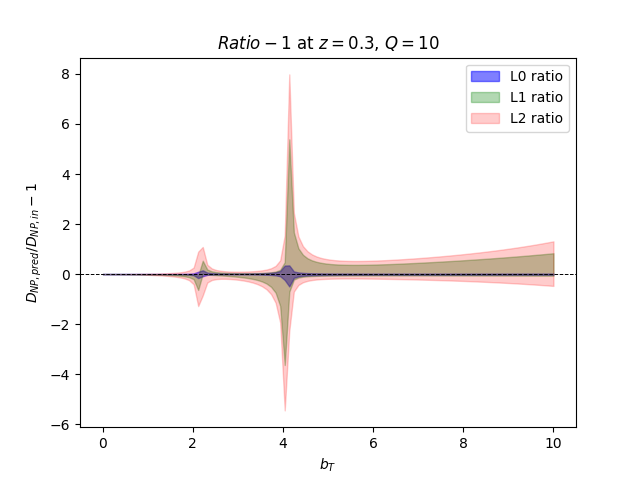
\includegraphics[width=\textwidth]{Images/unc_levels/RealVsPredRatio_D_NP_Q_10_z_0.3.png}
        \caption{$z = 0.3$}
    \end{minipage}\hfill
    \begin{minipage}{0.45\textwidth}
        \centering
        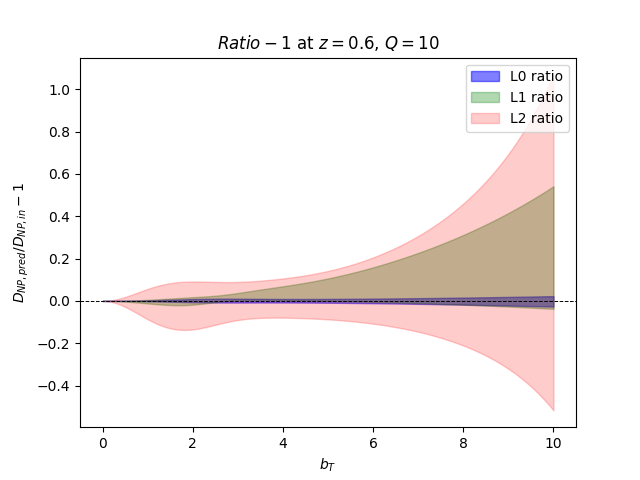
\includegraphics[width=\textwidth]{Images/unc_levels/RealVsPredRatio_D_NP_Q_10_z_0.6.png}
        \caption{$z=0.6$}
    \end{minipage}
    \caption{$\frac{D_{NP, pred}}{D_{NP, in}}-1$ at $Q=10 GeV$}
    \end{figure}

    \begin{figure}[H]
    \centering
    \begin{minipage}{0.45\textwidth}
        \centering
        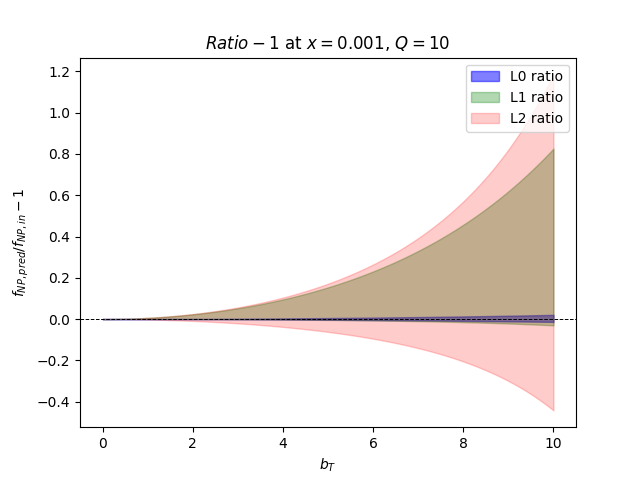
\includegraphics[width=\textwidth]{Images/unc_levels/RealVsPredRatio_f_NP_Q_10_x_0.001.png}
        \caption{$x = 0.001$}
    \end{minipage}\hfill
    \begin{minipage}{0.45\textwidth}
        \centering
        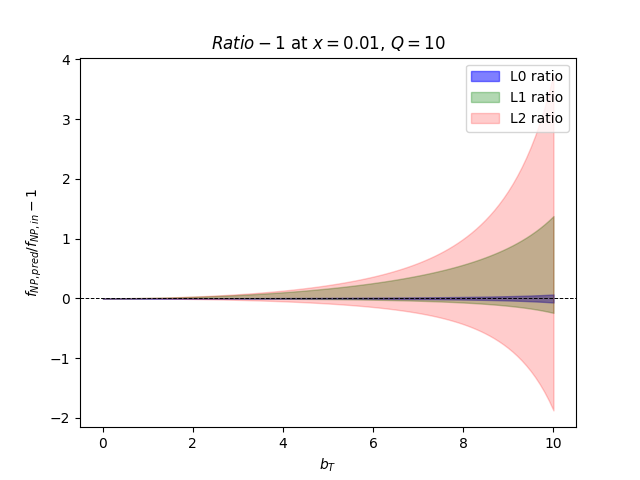
\includegraphics[width=\textwidth]{Images/unc_levels/RealVsPredRatio_f_NP_Q_10_x_0.01.png}
        \caption{$x=0.01$}
    \end{minipage}
    \begin{minipage}{0.45\textwidth}
        \centering
        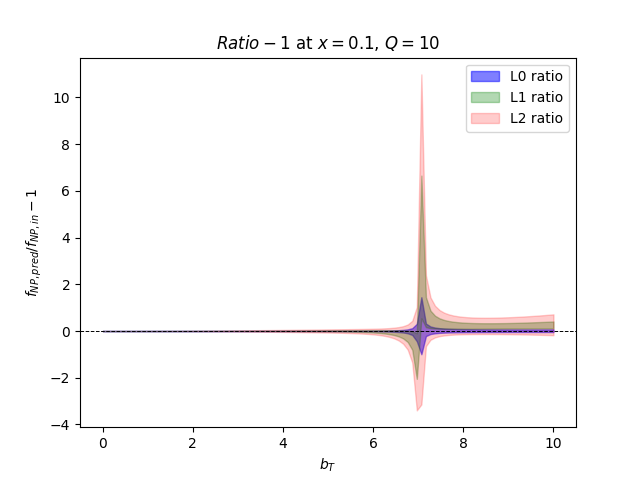
\includegraphics[width=\textwidth]{Images/unc_levels/RealVsPredRatio_f_NP_Q_10_x_0.1.png}
        \caption{$x=0.1$}
    \end{minipage}
    \caption{$\frac{f_{NP, pred}}{f_{NP, in}}-1$ at $Q=10 GeV$}
    \end{figure}

    I plot seguenti rappresentano gli stessi risultati a $Q=2GeV$
    
    \begin{figure}[H]
    \centering
    \begin{minipage}{0.45\textwidth}
        \centering
        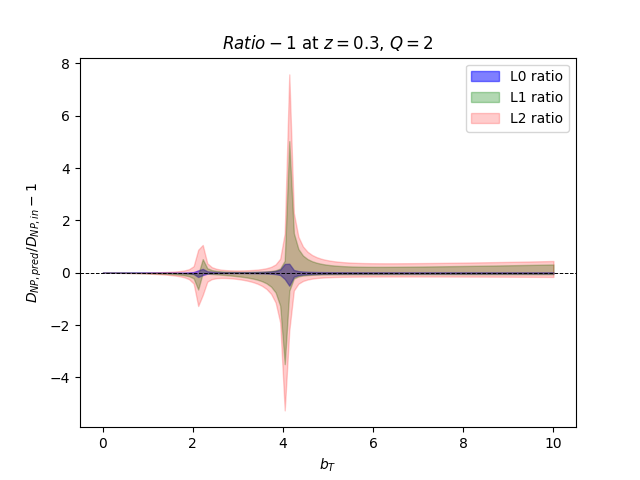
\includegraphics[width=\textwidth]{Images/unc_levels/RealVsPredRatio_D_NP_Q_2_z_0.3.png}
        \caption{$z = 0.3$}
    \end{minipage}\hfill
    \begin{minipage}{0.45\textwidth}
        \centering
        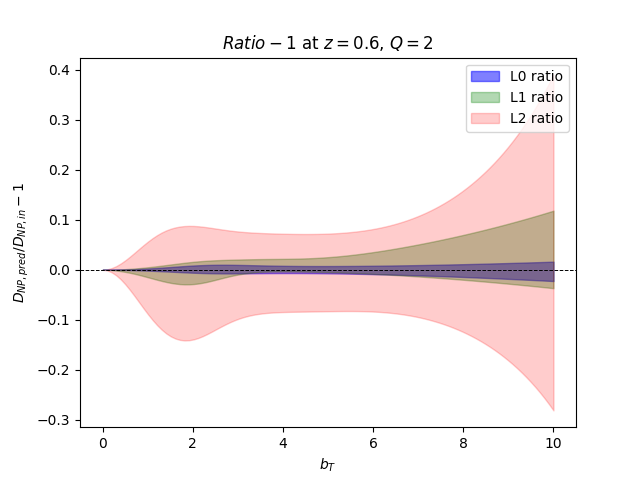
\includegraphics[width=\textwidth]{Images/unc_levels/RealVsPredRatio_D_NP_Q_2_z_0.6.png}
        \caption{$z=0.6$}
    \end{minipage}
    \caption{$\frac{D_{NP, pred}}{D_{NP, in}}-1$ at $Q=2 GeV$}
    \end{figure}

    \begin{figure}[H]
    \centering
    \begin{minipage}{0.45\textwidth}
        \centering
        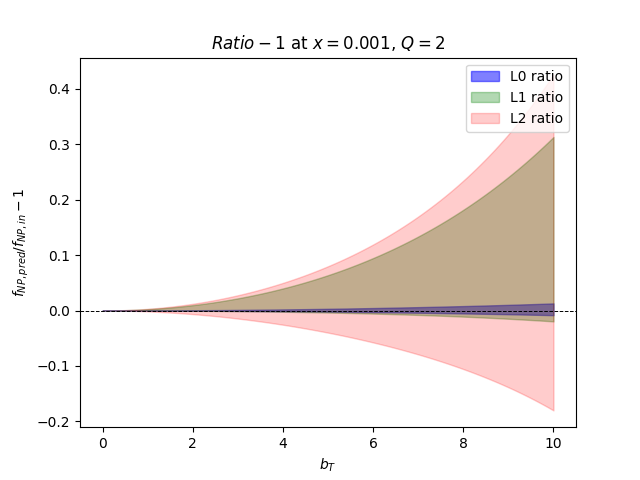
\includegraphics[width=\textwidth]{Images/unc_levels/RealVsPredRatio_f_NP_Q_2_x_0.001.png}
        \caption{$x = 0.001$}
    \end{minipage}\hfill
    \begin{minipage}{0.45\textwidth}
        \centering
        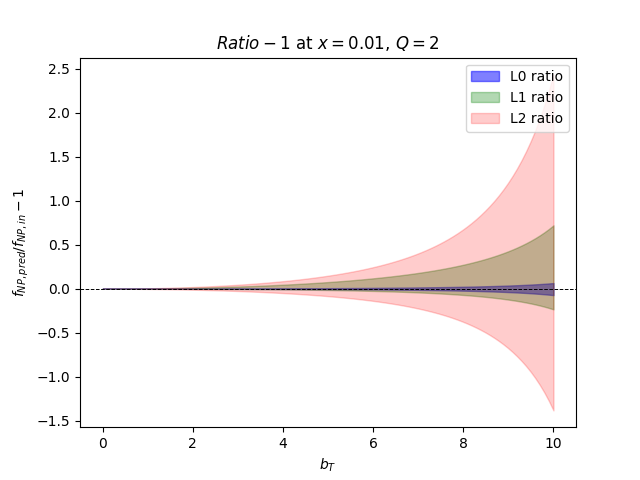
\includegraphics[width=\textwidth]{Images/unc_levels/RealVsPredRatio_f_NP_Q_2_x_0.01.png}
        \caption{$x=0.01$}
    \end{minipage}
    \begin{minipage}{0.45\textwidth}
        \centering
        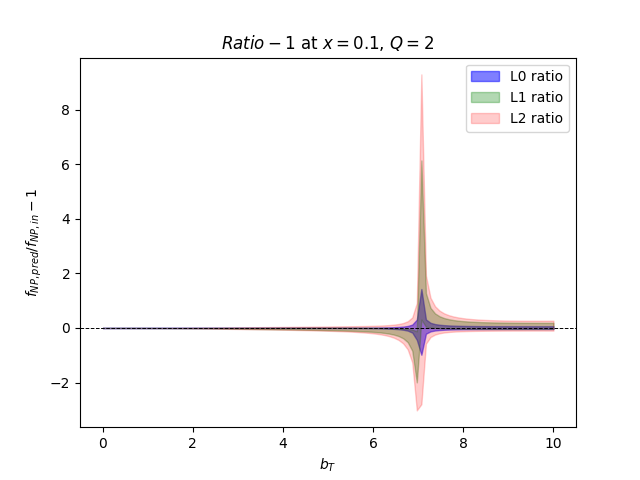
\includegraphics[width=\textwidth]{Images/unc_levels/RealVsPredRatio_f_NP_Q_2_x_0.1.png}
        \caption{$x=0.1$}
    \end{minipage}
    \caption{$\frac{f_{NP, pred}}{f_{NP, in}}-1$ at $Q=2 GeV$}
    \end{figure}


    \item \textbf{Rapporto tra le incertezze: } Possiamo anche studiare il rapporto tra le incertezze data dai fit sui dati al L0, L1 e L2 in ogni punto di $b_T$ considerato per avere un andamemto che rappresenti la percentuale di ogni incertezza rispetto all'incertezza totale.

    \begin{figure}[H]
    \centering
    \begin{minipage}{0.45\textwidth}
        \centering
        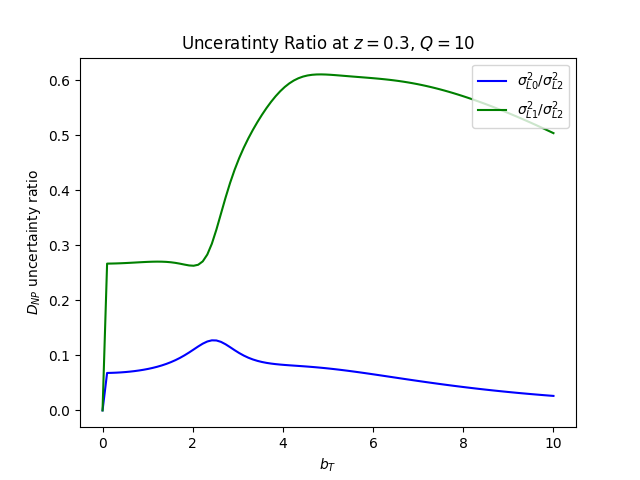
\includegraphics[width=\textwidth]{Images/unc_ratios/unc_ratio_D_NP_Q_10_z_0.3.png}
        \caption{$z = 0.3$}
    \end{minipage}\hfill
    \begin{minipage}{0.45\textwidth}
        \centering
        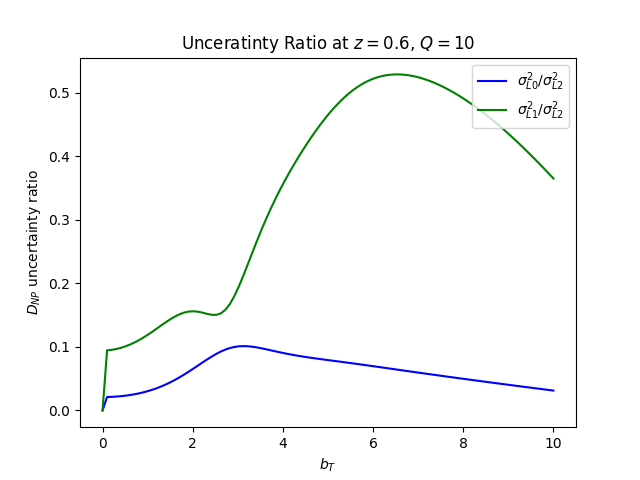
\includegraphics[width=\textwidth]{Images/unc_ratios/unc_ratio_D_NP_Q_10_z_0.6.png}
        \caption{$z=0.6$}
    \end{minipage}
    \caption{$D_{NP, pred}$ uncertainty ratios at $Q = 10 GeV$}
    \end{figure}

    \begin{figure}[H]
    \centering
    \begin{minipage}{0.45\textwidth}
        \centering
        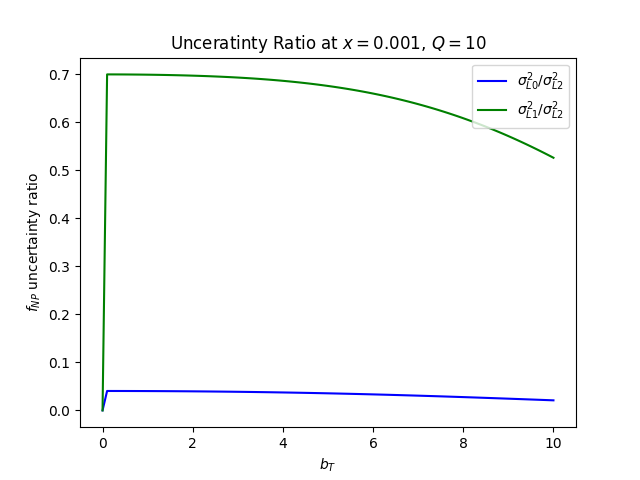
\includegraphics[width=\textwidth]{Images/unc_ratios/unc_ratio_f_NP_Q_10_x_0.001.png}
        \caption{$x = 0.001$}
    \end{minipage}\hfill
    \begin{minipage}{0.45\textwidth}
        \centering
        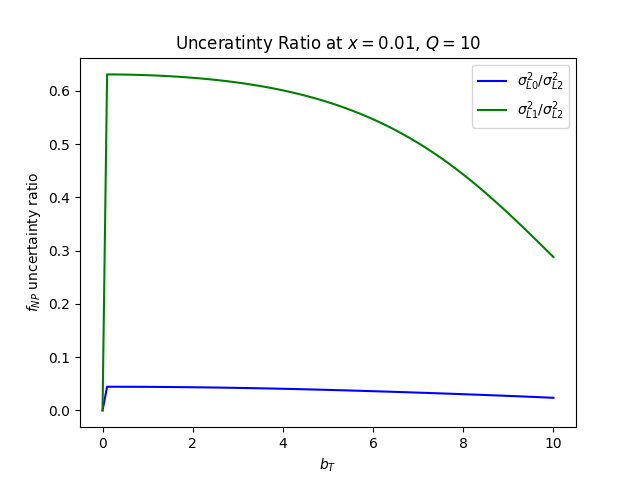
\includegraphics[width=\textwidth]{Images/unc_ratios/unc_ratio_f_NP_Q_10_x_0.01.png}
        \caption{$x=0.01$}
    \end{minipage}
    \begin{minipage}{0.45\textwidth}
        \centering
        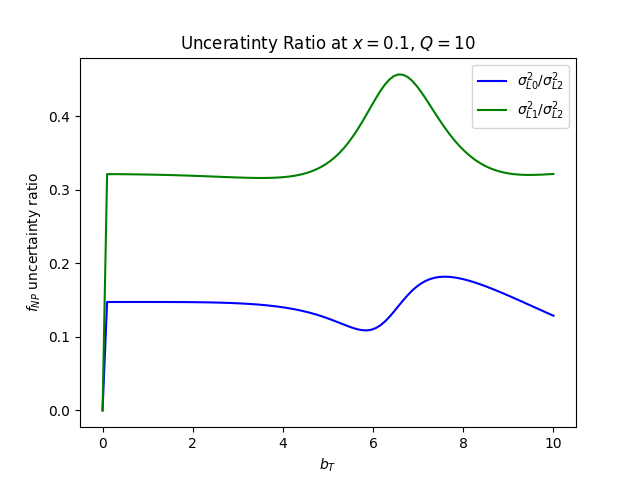
\includegraphics[width=\textwidth]{Images/unc_ratios/unc_ratio_f_NP_Q_10_x_0.1.png}
        \caption{$x=0.1$}
    \end{minipage}
    \caption{$f_{NP, pred}$ uncertainty ratios at $Q = 10 GeV$}
    \end{figure}

    Seguono gli stessi plot a $Q=2 GeV$
       \begin{figure}[H]
    \centering
    \begin{minipage}{0.45\textwidth}
        \centering
        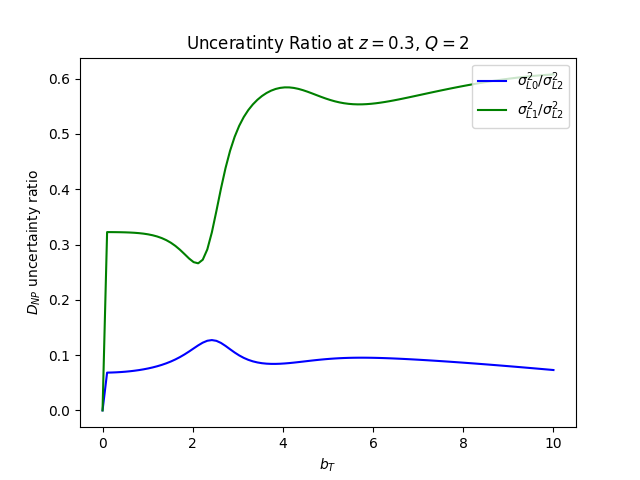
\includegraphics[width=\textwidth]{Images/unc_ratios/unc_ratio_D_NP_Q_2_z_0.3.png}
        \caption{$z = 0.3$}
    \end{minipage}\hfill
    \begin{minipage}{0.45\textwidth}
        \centering
        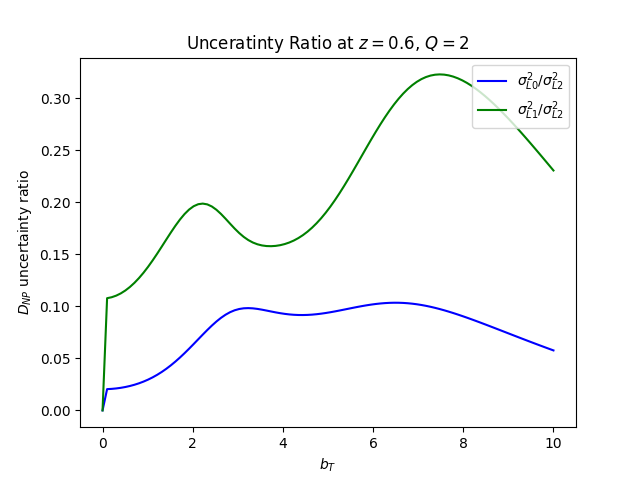
\includegraphics[width=\textwidth]{Images/unc_ratios/unc_ratio_D_NP_Q_2_z_0.6.png}
        \caption{$z=0.6$}
    \end{minipage}
    \caption{$D_{NP, pred}$ uncertainty ratios at $Q = 10 GeV$}
    \end{figure}

    \begin{figure}[H]
    \centering
    \begin{minipage}{0.45\textwidth}
        \centering
        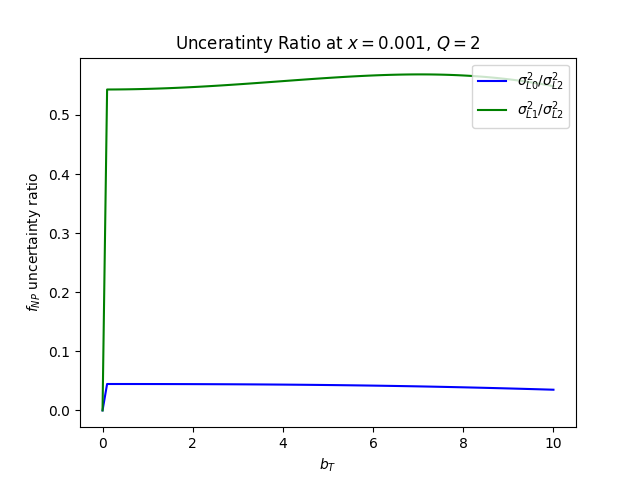
\includegraphics[width=\textwidth]{Images/unc_ratios/unc_ratio_f_NP_Q_2_x_0.001.png}
        \caption{$x = 0.001$}
    \end{minipage}\hfill
    \begin{minipage}{0.45\textwidth}
        \centering
        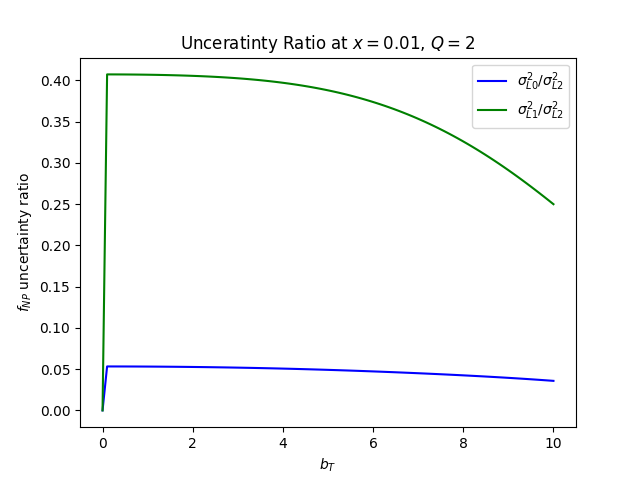
\includegraphics[width=\textwidth]{Images/unc_ratios/unc_ratio_f_NP_Q_2_x_0.01.png}
        \caption{$x=0.01$}
    \end{minipage}
    \begin{minipage}{0.45\textwidth}
        \centering
        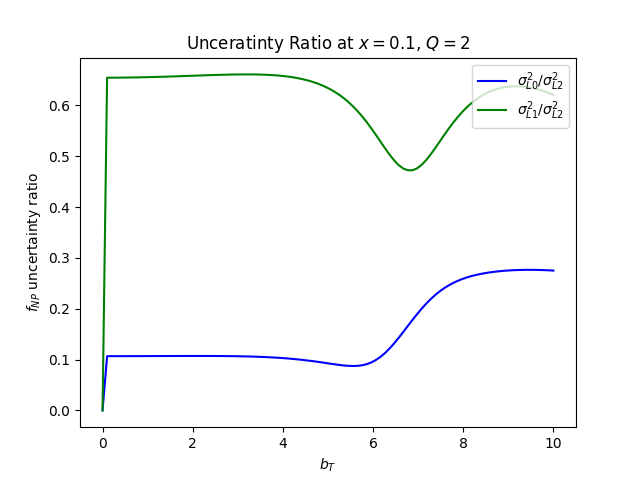
\includegraphics[width=\textwidth]{Images/unc_ratios/unc_ratio_f_NP_Q_2_x_0.1.png}
        \caption{$x=0.1$}
    \end{minipage}
    \caption{$f_{NP, pred}$ uncertainty ratios at $Q = 10 GeV$}
    \end{figure}
\end{itemize}

\section{Domande}
\begin{itemize}
    \item \textbf{diagrammi tagliati:} Ho ancora dei problemi sull'interpretazione di certi diagrammi tagliati che compaiono nella descrizione delle sezioni d'urto

    \item \textbf{errori con/senza taglio degli outliers:} le barre di errore che si vedono nei plot sono ricavate senza escludere nessuna replica (escludiamo solo le repliche non convergenti). Potremmo fare un test che risponde alla domanda "cosa cambia nelle barre d'errore se escludo gli outliers?"

    \item \textbf{scala logaritmica:} può avere senso usare la scala logaritmica in $y$ nei casi in cui l'incertezza diventa molto alta? Oppure (come nell'articolo NNPDF) conviene troncare il plot a certi valori di $y$? 

    \item \textbf{incertezza totale:} l'incertezza totale su una certa distribuzione corrisponde all'incertezza sperimentale (L2)?
\end{itemize}
\end{document}